% Options for packages loaded elsewhere
\PassOptionsToPackage{unicode}{hyperref}
\PassOptionsToPackage{hyphens}{url}
%
\documentclass[
]{article}
\usepackage{lmodern}
\usepackage{amssymb,amsmath}
\usepackage{ifxetex,ifluatex}
\ifnum 0\ifxetex 1\fi\ifluatex 1\fi=0 % if pdftex
  \usepackage[T1]{fontenc}
  \usepackage[utf8]{inputenc}
  \usepackage{textcomp} % provide euro and other symbols
\else % if luatex or xetex
  \usepackage{unicode-math}
  \defaultfontfeatures{Scale=MatchLowercase}
  \defaultfontfeatures[\rmfamily]{Ligatures=TeX,Scale=1}
\fi
% Use upquote if available, for straight quotes in verbatim environments
\IfFileExists{upquote.sty}{\usepackage{upquote}}{}
\IfFileExists{microtype.sty}{% use microtype if available
  \usepackage[]{microtype}
  \UseMicrotypeSet[protrusion]{basicmath} % disable protrusion for tt fonts
}{}
\makeatletter
\@ifundefined{KOMAClassName}{% if non-KOMA class
  \IfFileExists{parskip.sty}{%
    \usepackage{parskip}
  }{% else
    \setlength{\parindent}{0pt}
    \setlength{\parskip}{6pt plus 2pt minus 1pt}}
}{% if KOMA class
  \KOMAoptions{parskip=half}}
\makeatother
\usepackage{xcolor}
\IfFileExists{xurl.sty}{\usepackage{xurl}}{} % add URL line breaks if available
\IfFileExists{bookmark.sty}{\usepackage{bookmark}}{\usepackage{hyperref}}
\hypersetup{
  pdftitle={Cardiotocograms Classification in RStudio},
  pdfauthor={by o.cardec},
  hidelinks,
  pdfcreator={LaTeX via pandoc}}
\urlstyle{same} % disable monospaced font for URLs
\usepackage[margin=1in]{geometry}
\usepackage{color}
\usepackage{fancyvrb}
\newcommand{\VerbBar}{|}
\newcommand{\VERB}{\Verb[commandchars=\\\{\}]}
\DefineVerbatimEnvironment{Highlighting}{Verbatim}{commandchars=\\\{\}}
% Add ',fontsize=\small' for more characters per line
\usepackage{framed}
\definecolor{shadecolor}{RGB}{248,248,248}
\newenvironment{Shaded}{\begin{snugshade}}{\end{snugshade}}
\newcommand{\AlertTok}[1]{\textcolor[rgb]{0.94,0.16,0.16}{#1}}
\newcommand{\AnnotationTok}[1]{\textcolor[rgb]{0.56,0.35,0.01}{\textbf{\textit{#1}}}}
\newcommand{\AttributeTok}[1]{\textcolor[rgb]{0.77,0.63,0.00}{#1}}
\newcommand{\BaseNTok}[1]{\textcolor[rgb]{0.00,0.00,0.81}{#1}}
\newcommand{\BuiltInTok}[1]{#1}
\newcommand{\CharTok}[1]{\textcolor[rgb]{0.31,0.60,0.02}{#1}}
\newcommand{\CommentTok}[1]{\textcolor[rgb]{0.56,0.35,0.01}{\textit{#1}}}
\newcommand{\CommentVarTok}[1]{\textcolor[rgb]{0.56,0.35,0.01}{\textbf{\textit{#1}}}}
\newcommand{\ConstantTok}[1]{\textcolor[rgb]{0.00,0.00,0.00}{#1}}
\newcommand{\ControlFlowTok}[1]{\textcolor[rgb]{0.13,0.29,0.53}{\textbf{#1}}}
\newcommand{\DataTypeTok}[1]{\textcolor[rgb]{0.13,0.29,0.53}{#1}}
\newcommand{\DecValTok}[1]{\textcolor[rgb]{0.00,0.00,0.81}{#1}}
\newcommand{\DocumentationTok}[1]{\textcolor[rgb]{0.56,0.35,0.01}{\textbf{\textit{#1}}}}
\newcommand{\ErrorTok}[1]{\textcolor[rgb]{0.64,0.00,0.00}{\textbf{#1}}}
\newcommand{\ExtensionTok}[1]{#1}
\newcommand{\FloatTok}[1]{\textcolor[rgb]{0.00,0.00,0.81}{#1}}
\newcommand{\FunctionTok}[1]{\textcolor[rgb]{0.00,0.00,0.00}{#1}}
\newcommand{\ImportTok}[1]{#1}
\newcommand{\InformationTok}[1]{\textcolor[rgb]{0.56,0.35,0.01}{\textbf{\textit{#1}}}}
\newcommand{\KeywordTok}[1]{\textcolor[rgb]{0.13,0.29,0.53}{\textbf{#1}}}
\newcommand{\NormalTok}[1]{#1}
\newcommand{\OperatorTok}[1]{\textcolor[rgb]{0.81,0.36,0.00}{\textbf{#1}}}
\newcommand{\OtherTok}[1]{\textcolor[rgb]{0.56,0.35,0.01}{#1}}
\newcommand{\PreprocessorTok}[1]{\textcolor[rgb]{0.56,0.35,0.01}{\textit{#1}}}
\newcommand{\RegionMarkerTok}[1]{#1}
\newcommand{\SpecialCharTok}[1]{\textcolor[rgb]{0.00,0.00,0.00}{#1}}
\newcommand{\SpecialStringTok}[1]{\textcolor[rgb]{0.31,0.60,0.02}{#1}}
\newcommand{\StringTok}[1]{\textcolor[rgb]{0.31,0.60,0.02}{#1}}
\newcommand{\VariableTok}[1]{\textcolor[rgb]{0.00,0.00,0.00}{#1}}
\newcommand{\VerbatimStringTok}[1]{\textcolor[rgb]{0.31,0.60,0.02}{#1}}
\newcommand{\WarningTok}[1]{\textcolor[rgb]{0.56,0.35,0.01}{\textbf{\textit{#1}}}}
\usepackage{graphicx}
\makeatletter
\def\maxwidth{\ifdim\Gin@nat@width>\linewidth\linewidth\else\Gin@nat@width\fi}
\def\maxheight{\ifdim\Gin@nat@height>\textheight\textheight\else\Gin@nat@height\fi}
\makeatother
% Scale images if necessary, so that they will not overflow the page
% margins by default, and it is still possible to overwrite the defaults
% using explicit options in \includegraphics[width, height, ...]{}
\setkeys{Gin}{width=\maxwidth,height=\maxheight,keepaspectratio}
% Set default figure placement to htbp
\makeatletter
\def\fps@figure{htbp}
\makeatother
\setlength{\emergencystretch}{3em} % prevent overfull lines
\providecommand{\tightlist}{%
  \setlength{\itemsep}{0pt}\setlength{\parskip}{0pt}}
\setcounter{secnumdepth}{-\maxdimen} % remove section numbering
\ifluatex
  \usepackage{selnolig}  % disable illegal ligatures
\fi

\title{Cardiotocograms Classification in RStudio}
\author{by o.cardec}
\date{12/6/2020}

\begin{document}
\maketitle

\hypertarget{introduction}{%
\subsubsection{Introduction}\label{introduction}}

Cardiotocograms, also known as CTGs, have been instrumental within
clinical medicine for a long time. Obstetricians use these measurements
and classifications to obtain detailed information and intelligence
about newborns and their mother prior and during labor. In 2018, an
article presented through the Journal of Clinical Medicine detailed the
practicality of CTGs. The same noted that interpretations of these
censorial readings is mainly attributed to the observer; which creates
challenges of consistency of interpretations and defies the human
naked-eye. Questions like what happens, if or when, the interpreter
misses a key detail? Furthermore, what time-sensitive conditions may the
measurements uncover, requiring immediate actions are few examples of
concerns posed by the continuous practice of merely optical assessments
of a CTG (Zhao, Zhang \& Deng, 2018).

The following report presents an assessment of CTGs using the
conditional inference tree (ctree) model within RStudio. The same shows
how the algorithm expedites and enhances the interpretation of CTG
readings while appraising multiple fetal readings simultaneously.
Moreover, the study aims to identify potential hidden patters which may
require further attention.

The data-frame to be analyzed comes for the UCI Machine Learning
Repository, and it consists of measurements of fetal heart rate (FHR)
and uterine contraction (UC) as identified and recorded by
cardiotocograms. It contains 2126 observations and 23 variables. Each
diagnostic attribute within these CTGs were automatically processed and
measured. Finally, for supervised learning purposes, all CTGs were
classified by three subject matter experts, and under unanimity,
assigned them with response-labels based on the fetal state and/or
morphological detected patterns (Dua, \& Graff, 2019).

\textbf{Data Dictionary}

\begin{itemize}
\tightlist
\item
  LB: FHR baseline (beats per minute)\\
\item
  AC: Number of accelerations per second
\item
  FM: Number of fetal movements per second
\item
  UC: Number of uterine contractions per second
\item
  DL: Number of light decelerations per second
\item
  DS: Number of severe decelerations per second
\item
  DP: Number of prolonged decelerations per second
\item
  ASTV: Percentage of time with abnormal short-term variability
\item
  MSTV: Mean value of short term variability
\item
  ALTV: Percentage of time with abnormal long-term variability
\item
  MLTV: Mean value of long -erm variability
\item
  Width: Width of FHR histogram
\item
  Min: Minimum of FHR histogram
\item
  Max: Maximum of FHR histogram
\item
  Nmax: Number of histogram peaks
\item
  Nzeros: Number of histogram zeros
\item
  Mode: Histogram mode
\item
  Mean - Histogram mean
\item
  Median - Histogram median
\item
  Variance - Histogram variance
\item
  Tendency - Histogram tendency
\item
  CLASS - FHR pattern class code (1 to 10)
\item
  NSP - Fetal state class code (N=normal; S = suspect; P=pathologic
\end{itemize}

As observed, the above list includes unique CTG measurements,
statistical attributes as well as observations from some of the recorded
variables. The last two variables, CLASS and NSP, represent the
previously mentioned classification and response-labeling conducted by
the obstetricians.

\hypertarget{exploratory-analysis}{%
\subsubsection{Exploratory Analysis}\label{exploratory-analysis}}

The given cardiotocography.csv file was loaded and vectored as ctg. A
look into the structure of the data-frame confirms some of the variables
and information obtained from the repository and .csv file itself. The
2126 observations are a mix of formatted integers and numeric values. A
glimpse over these represented values highlight few transformation
options. Case in point, the targeted variable, which is the NSP, will
need to get converted to a factor. Other variables like FM, DP, or ALTV
may be representative of asymmetrical distributions. Furthermore, a
variable like DS which appears to have only one type of response, making
it incomparable for classification purposes.

\begin{verbatim}
##        LB              AC                 FM                 UC          
##  Min.   :106.0   Min.   :0.000000   Min.   :0.000000   Min.   :0.000000  
##  1st Qu.:126.0   1st Qu.:0.000000   1st Qu.:0.000000   1st Qu.:0.002000  
##  Median :133.0   Median :0.002000   Median :0.000000   Median :0.004000  
##  Mean   :133.3   Mean   :0.003178   Mean   :0.009481   Mean   :0.004366  
##  3rd Qu.:140.0   3rd Qu.:0.006000   3rd Qu.:0.003000   3rd Qu.:0.007000  
##  Max.   :160.0   Max.   :0.019000   Max.   :0.481000   Max.   :0.015000  
##        DL                 DS                  DP                 ASTV      
##  Min.   :0.000000   Min.   :0.000e+00   Min.   :0.0000000   Min.   :12.00  
##  1st Qu.:0.000000   1st Qu.:0.000e+00   1st Qu.:0.0000000   1st Qu.:32.00  
##  Median :0.000000   Median :0.000e+00   Median :0.0000000   Median :49.00  
##  Mean   :0.001889   Mean   :3.293e-06   Mean   :0.0001585   Mean   :46.99  
##  3rd Qu.:0.003000   3rd Qu.:0.000e+00   3rd Qu.:0.0000000   3rd Qu.:61.00  
##  Max.   :0.015000   Max.   :1.000e-03   Max.   :0.0050000   Max.   :87.00  
##       MSTV            ALTV             MLTV            Width       
##  Min.   :0.200   Min.   : 0.000   Min.   : 0.000   Min.   :  3.00  
##  1st Qu.:0.700   1st Qu.: 0.000   1st Qu.: 4.600   1st Qu.: 37.00  
##  Median :1.200   Median : 0.000   Median : 7.400   Median : 67.50  
##  Mean   :1.333   Mean   : 9.847   Mean   : 8.188   Mean   : 70.45  
##  3rd Qu.:1.700   3rd Qu.:11.000   3rd Qu.:10.800   3rd Qu.:100.00  
##  Max.   :7.000   Max.   :91.000   Max.   :50.700   Max.   :180.00  
##       Min              Max           Nmax            Nzeros       
##  Min.   : 50.00   Min.   :122   Min.   : 0.000   Min.   : 0.0000  
##  1st Qu.: 67.00   1st Qu.:152   1st Qu.: 2.000   1st Qu.: 0.0000  
##  Median : 93.00   Median :162   Median : 3.000   Median : 0.0000  
##  Mean   : 93.58   Mean   :164   Mean   : 4.068   Mean   : 0.3236  
##  3rd Qu.:120.00   3rd Qu.:174   3rd Qu.: 6.000   3rd Qu.: 0.0000  
##  Max.   :159.00   Max.   :238   Max.   :18.000   Max.   :10.0000  
##       Mode            Mean           Median         Variance     
##  Min.   : 60.0   Min.   : 73.0   Min.   : 77.0   Min.   :  0.00  
##  1st Qu.:129.0   1st Qu.:125.0   1st Qu.:129.0   1st Qu.:  2.00  
##  Median :139.0   Median :136.0   Median :139.0   Median :  7.00  
##  Mean   :137.5   Mean   :134.6   Mean   :138.1   Mean   : 18.81  
##  3rd Qu.:148.0   3rd Qu.:145.0   3rd Qu.:148.0   3rd Qu.: 24.00  
##  Max.   :187.0   Max.   :182.0   Max.   :186.0   Max.   :269.00  
##     Tendency           CLASS            NSP       
##  Min.   :-1.0000   Min.   : 1.00   Min.   :1.000  
##  1st Qu.: 0.0000   1st Qu.: 2.00   1st Qu.:1.000  
##  Median : 0.0000   Median : 4.00   Median :1.000  
##  Mean   : 0.3203   Mean   : 4.51   Mean   :1.304  
##  3rd Qu.: 1.0000   3rd Qu.: 7.00   3rd Qu.:1.000  
##  Max.   : 1.0000   Max.   :10.00   Max.   :3.000
\end{verbatim}

\emph{Figure 1.1 -- NSP, as the response variable, will be converted to
a factor}\\
The above illustration expands and corroborates other aspects within the
data. Case in point, judging by the numbers, Width, Min, Max, Nmax,
Nzeros, Mode, Mean, Median, Variance, and Tendency appear to be
statistical results of a measurement. Also, the variance across
distributions is evident, thus, extra steps will have to be taken during
the pre-processing phase. Lastly, there are no NA values within the set.

After reviewing the statistical attributes of the data set, a histogram
was built to represent the LB variable. Per the data dictionary, this
particular attribute is the most influential attribute of the set. The
image in figure 1.2 shows how equally distributed the LB attribute is,
and by the featured frequency, the mean will most likely fall between
130-135 heart-beats per minute.

\includegraphics{CTREE_RMarkdown_files/figure-latex/LBdistribution-1.pdf}

\emph{Figure 1.2 -- Fetal heart hate baseline (LB variable) is fairly
distributed.}

Motivated by the variability of the baseline distribution, a deeper look
was taken to identify out of the represented observations which ones
were outside the 2-standard deviation (s.d.) ranges. Figure 1.3,
portrays what the developed code captured. It shows the values
associated to 1 or 2 s.d.s' boundaries, and how some of the readings
exceed such limits.

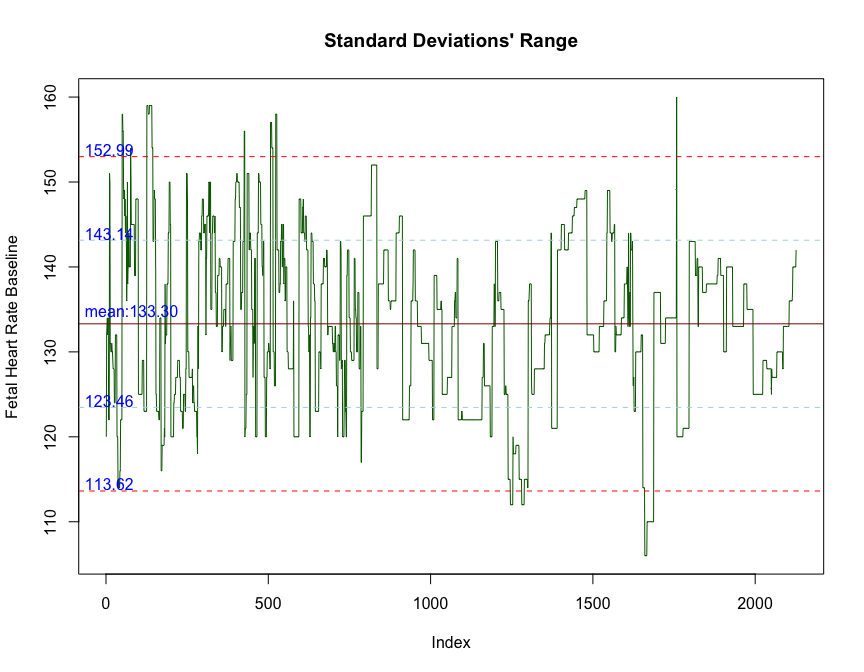
\includegraphics{CTREE_RMarkdown_files/figure-latex/LB distro boundaries-1.pdf}
\emph{Figure 1.3 -- Graphical display of LB's 1 \& 2 standard
deviations.}

Further calculation, like the one below, shows how critical this reading
resulted, given that those readings within 2 s.d. account for over 96\%
of the studied observations. That said, this does not imply the
contained readings are one way or the other (normal, suspect, or
pathologic), but instead shows the usability of these quantified
observations.

\begin{verbatim}
## [1] 83
\end{verbatim}

\begin{verbatim}
## [1] 96.1
\end{verbatim}

Considering the findings through the EDA process, and explanatory
details from the data source, the variables that were not part of the
original collection were excluded. After further inquiry, these
characteristics and calculations were related to the FHR baseline
histogram made by the analytical software used by the dataset
originators (Zhao, Zhang \& Deng, 2018). Initially, the CLASS variable
was converted to a factor and all of its 10 levels renamed.
Unfortunately, this variable also resulted to be a classification
conducted by the medical practicioners, and contributed to overfitting
of the model, thus forcing to reassess the development approach. That
said, the CLASS variable was used as a guide for interpretation, but not
included on the final set of variables to test within the model.
Besides, the NSP variable was transformed to a factor, and its levels
renamed to normal, suspect, and pathologic. Figure 1.4 gives a brief
look of some of the variables and their respective distribution
characteristics.

\begin{Shaded}
\begin{Highlighting}[]
\CommentTok{\# Distributions preview}
\NormalTok{ctg[,}\DecValTok{1}\SpecialCharTok{:}\DecValTok{12}\NormalTok{] }\SpecialCharTok{\%\textgreater{}\%} 
  \FunctionTok{gather}\NormalTok{() }\SpecialCharTok{\%\textgreater{}\%}                             
  \FunctionTok{ggplot}\NormalTok{(}\FunctionTok{aes}\NormalTok{(value)) }\SpecialCharTok{+}
  \FunctionTok{theme\_light}\NormalTok{() }\SpecialCharTok{+} \FunctionTok{labs}\NormalTok{( }\AttributeTok{title=}\StringTok{"FHR Measurement Distributions"}\NormalTok{)}\SpecialCharTok{+}
  \FunctionTok{theme}\NormalTok{(}\AttributeTok{axis.text.x =} \FunctionTok{element\_text}\NormalTok{(}\AttributeTok{angle=}\DecValTok{90}\NormalTok{)) }\SpecialCharTok{+}                 
  \FunctionTok{facet\_wrap}\NormalTok{(}\SpecialCharTok{\textasciitilde{}}\NormalTok{ key, }\AttributeTok{scales =} \StringTok{"free"}\NormalTok{, }\AttributeTok{shrink =} \ConstantTok{TRUE}\NormalTok{) }\SpecialCharTok{+}  
  \FunctionTok{geom\_bar}\NormalTok{(}\AttributeTok{mapping =} \FunctionTok{aes}\NormalTok{(value), }
           \AttributeTok{color=}\StringTok{"darkblue"}\NormalTok{, }\AttributeTok{fill=}\StringTok{"lightgrey"}\NormalTok{)}
\end{Highlighting}
\end{Shaded}

\begin{verbatim}
## Warning: attributes are not identical across measure variables;
## they will be dropped
\end{verbatim}

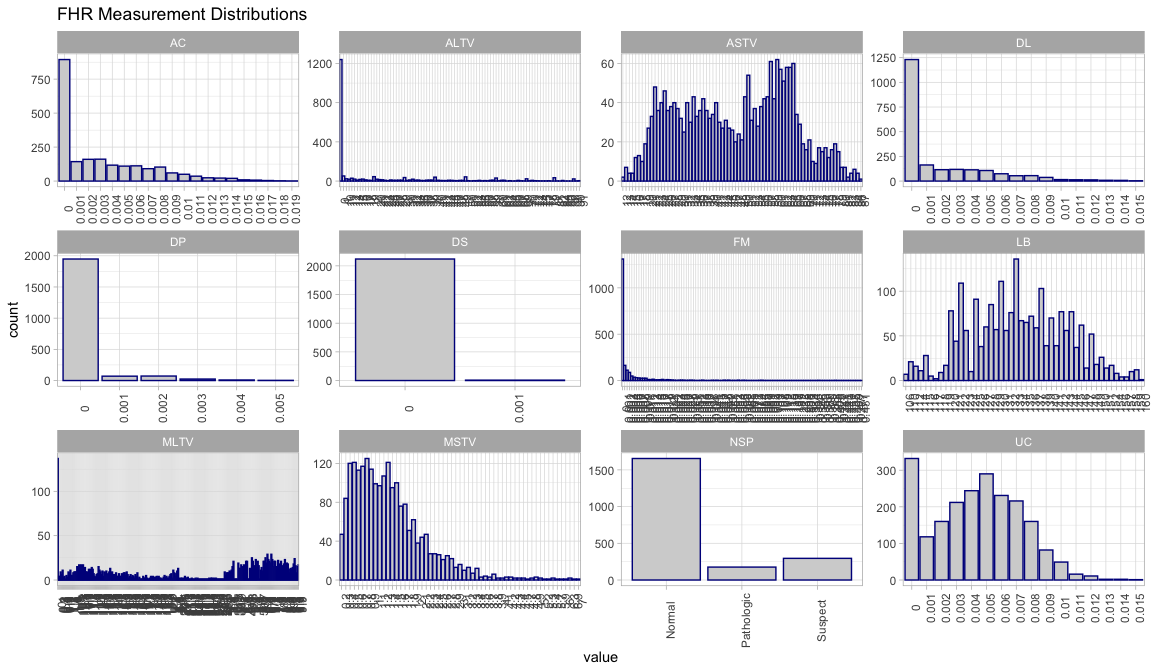
\includegraphics{CTREE_RMarkdown_files/figure-latex/dismatrix-1.pdf}
\emph{Figure 1.4 -- Dataset transformed.}

\textbf{Algorithm Intuition:}

As previously stated, the conditional inference tree (ctree) is the
algorithm to employ for this dataset classification. The objective is to
use the model for identification of those independent variables with the
greatest influence against the response variable. Author, Torsten
Hothorn, summarizes the algorithm behind the ctree as follow, ``A
conditional inference trees estimate a regression relationship by binary
recursive partitioning in a conditional inference framework (2006).
Hothorn explains that first ``the algorithm tests the sample for
hypothesis of independence between the independent variables and the
response''. If the hypothesis cannot be rejected the process stops.
Conversely, it selects the variable with the strongest measured
association (measured by the corresponding p-value). Secondly, it
implements a binary decision and split in the selected variable, and
recursively continues this process until all observations get evaluated
(Hothon, 2006). The first step developing the model was setting a seed
and splitting the dataset into different samples to train and test the
model. After numerous evaluations, comparison of different simulations,
and accuracy appraisals, the dataset splitting proportions were set to
.70 and .30. Per figure 2.0, the probability weights for these subsets
were set to 70\%, and 30\% for the training and testing subsets,
respectively.

\begin{Shaded}
\begin{Highlighting}[]
\CommentTok{\# Creating the training and testing data subsets}
\FunctionTok{set.seed}\NormalTok{(}\DecValTok{1234}\NormalTok{)}
\NormalTok{ind }\OtherTok{\textless{}{-}} \FunctionTok{sample}\NormalTok{(}\DecValTok{2}\NormalTok{, }\FunctionTok{nrow}\NormalTok{(ctg), }\AttributeTok{replace =} \ConstantTok{TRUE}\NormalTok{, }\AttributeTok{prob =} \FunctionTok{c}\NormalTok{(}\FloatTok{0.70}\NormalTok{, }\FloatTok{0.30}\NormalTok{))}
\NormalTok{train.data }\OtherTok{\textless{}{-}}\NormalTok{ ctg[ind }\SpecialCharTok{==} \DecValTok{1}\NormalTok{, ]}
\NormalTok{test.data }\OtherTok{\textless{}{-}}\NormalTok{ ctg[ind }\SpecialCharTok{==} \DecValTok{2}\NormalTok{, ]}

\CommentTok{\# Runing the method against the train data subset}
\NormalTok{myFormula }\OtherTok{\textless{}{-}}\NormalTok{ NSP}\SpecialCharTok{\textasciitilde{}}\NormalTok{.}
\NormalTok{model }\OtherTok{\textless{}{-}} \FunctionTok{ctree}\NormalTok{(myFormula, }\AttributeTok{data =}\NormalTok{ train.data)}
\FunctionTok{print}\NormalTok{(model)}
\end{Highlighting}
\end{Shaded}

\begin{verbatim}
## 
## Model formula:
## NSP ~ LB + AC + FM + UC + DL + DS + DP + ASTV + MSTV + ALTV + 
##     MLTV
## 
## Fitted party:
## [1] root
## |   [2] DP <= 0.001
## |   |   [3] ALTV <= 68
## |   |   |   [4] ALTV <= 7
## |   |   |   |   [5] ASTV <= 73
## |   |   |   |   |   [6] DL <= 0.008
## |   |   |   |   |   |   [7] DP <= 0
## |   |   |   |   |   |   |   [8] LB <= 149
## |   |   |   |   |   |   |   |   [9] AC <= 0.001
## |   |   |   |   |   |   |   |   |   [10] UC <= 0: Normal (n = 34, err = 14.7%)
## |   |   |   |   |   |   |   |   |   [11] UC > 0: Normal (n = 231, err = 3.5%)
## |   |   |   |   |   |   |   |   [12] AC > 0.001: Normal (n = 626, err = 0.3%)
## |   |   |   |   |   |   |   [13] LB > 149: Normal (n = 17, err = 35.3%)
## |   |   |   |   |   |   [14] DP > 0
## |   |   |   |   |   |   |   [15] MLTV <= 0.9: Normal (n = 7, err = 28.6%)
## |   |   |   |   |   |   |   [16] MLTV > 0.9
## |   |   |   |   |   |   |   |   [17] MLTV <= 8.8: Normal (n = 28, err = 0.0%)
## |   |   |   |   |   |   |   |   [18] MLTV > 8.8: Normal (n = 7, err = 28.6%)
## |   |   |   |   |   [19] DL > 0.008
## |   |   |   |   |   |   [20] ASTV <= 58: Normal (n = 35, err = 0.0%)
## |   |   |   |   |   |   [21] ASTV > 58: Pathologic (n = 25, err = 40.0%)
## |   |   |   |   [22] ASTV > 73: Pathologic (n = 11, err = 45.5%)
## |   |   |   [23] ALTV > 7
## |   |   |   |   [24] ASTV <= 80
## |   |   |   |   |   [25] ASTV <= 59
## |   |   |   |   |   |   [26] LB <= 137
## |   |   |   |   |   |   |   [27] MLTV <= 9.6: Normal (n = 72, err = 1.4%)
## |   |   |   |   |   |   |   [28] MLTV > 9.6: Normal (n = 26, err = 15.4%)
## |   |   |   |   |   |   [29] LB > 137: Normal (n = 111, err = 27.9%)
## |   |   |   |   |   [30] ASTV > 59
## |   |   |   |   |   |   [31] UC <= 0.003
## |   |   |   |   |   |   |   [32] AC <= 0.001
## |   |   |   |   |   |   |   |   [33] MSTV <= 0.6: Suspect (n = 92, err = 2.2%)
## |   |   |   |   |   |   |   |   [34] MSTV > 0.6: Suspect (n = 9, err = 33.3%)
## |   |   |   |   |   |   |   [35] AC > 0.001: Normal (n = 10, err = 50.0%)
## |   |   |   |   |   |   [36] UC > 0.003
## |   |   |   |   |   |   |   [37] LB <= 136
## |   |   |   |   |   |   |   |   [38] MLTV <= 5.1: Normal (n = 18, err = 0.0%)
## |   |   |   |   |   |   |   |   [39] MLTV > 5.1: Suspect (n = 11, err = 45.5%)
## |   |   |   |   |   |   |   [40] LB > 136
## |   |   |   |   |   |   |   |   [41] ASTV <= 69: Suspect (n = 22, err = 4.5%)
## |   |   |   |   |   |   |   |   [42] ASTV > 69: Normal (n = 8, err = 37.5%)
## |   |   |   |   [43] ASTV > 80: Pathologic (n = 13, err = 7.7%)
## |   |   [44] ALTV > 68
## |   |   |   [45] UC <= 0.001: Pathologic (n = 26, err = 0.0%)
## |   |   |   [46] UC > 0.001: Pathologic (n = 7, err = 28.6%)
## |   [47] DP > 0.001
## |   |   [48] ASTV <= 28: Normal (n = 12, err = 41.7%)
## |   |   [49] ASTV > 28
## |   |   |   [50] MLTV <= 5: Pathologic (n = 50, err = 6.0%)
## |   |   |   [51] MLTV > 5: Pathologic (n = 15, err = 26.7%)
## 
## Number of inner nodes:    25
## Number of terminal nodes: 26
\end{verbatim}

Per the illustration, the model consists of 25 inner nodes and 26
terminal nodes for a total of 51 nodes. The first split or branching to
the right occurs at the root where driven by DP ``prolonged
deceleration'' \textgreater{} 0.001, it groups 149 observations, with a
majority of pathologic cases distributed through nodes 47, 48, \& 49. To
the left of the root, DP readings of \textless0.001 decelerations are
furthered split by ALTV ``percentage of time with abnormal long term
variability'' of \textless68 to the left, and \textgreater68 to the
right to node 44. The footprint of the tree is significantly large,
illustrated on figure 2.1 Also, although the greater concentration of
pathologic cases are located at the right side of the tree, additional
pathologic cases are noticed on the left limbs, namely node 22, 21, and
15. As an observation, this is an example of irregular behaviors
potentially hidden to the human sight.

\begin{quote}
``Irregular behaviors, normally hidden to the naked-eye can easily get
identifed using algorightms''
\end{quote}

\begin{Shaded}
\begin{Highlighting}[]
\CommentTok{\# Tree visualization}
\FunctionTok{plot}\NormalTok{(model, }\AttributeTok{type=}\StringTok{"extended"}\NormalTok{, }\AttributeTok{ep\_args =} \FunctionTok{list}\NormalTok{(}\AttributeTok{justmin=}\DecValTok{10}\NormalTok{), }\AttributeTok{drop\_terminal=}\NormalTok{F, }\AttributeTok{tnex=}\FloatTok{1.2}\NormalTok{, }
     \AttributeTok{gp=}\FunctionTok{gpar}\NormalTok{(}\AttributeTok{fontsize =} \DecValTok{10}\NormalTok{, }\AttributeTok{col=}\StringTok{"dark blue"}\NormalTok{),}
     \AttributeTok{inner\_panel =} \FunctionTok{node\_inner}\NormalTok{(model, }\AttributeTok{fill=}\FunctionTok{c}\NormalTok{(}\StringTok{"light grey"}\NormalTok{,}\StringTok{"green"}\NormalTok{), }\AttributeTok{pval=}\NormalTok{T), }
     \AttributeTok{terminal\_panel=}\FunctionTok{node\_barplot}\NormalTok{(model, }\AttributeTok{fill=}\FunctionTok{c}\NormalTok{(}\DecValTok{3}\NormalTok{,}\DecValTok{7}\NormalTok{,}\DecValTok{2}\NormalTok{), }\AttributeTok{beside=}\NormalTok{T, }\AttributeTok{ymax=}\DecValTok{1}\NormalTok{, }\AttributeTok{rot =} \DecValTok{75}\NormalTok{, }
     \AttributeTok{just =} \FunctionTok{c}\NormalTok{(.}\DecValTok{95}\NormalTok{,.}\DecValTok{5}\NormalTok{), }\AttributeTok{ylines=}\NormalTok{T, }\AttributeTok{widths =} \DecValTok{3}\NormalTok{, }\AttributeTok{gap=}\FloatTok{0.05}\NormalTok{, }\AttributeTok{reverse=}\NormalTok{F, }\AttributeTok{id=}\NormalTok{T), }
     \AttributeTok{margins =} \FunctionTok{c}\NormalTok{(}\DecValTok{4}\NormalTok{,}\DecValTok{3}\NormalTok{, }\DecValTok{3}\NormalTok{, }\DecValTok{3}\NormalTok{), }
     \AttributeTok{main=}\StringTok{"Cardiotocography Data}\SpecialCharTok{\textbackslash{}n}\StringTok{ Conditional Inference Tree"}\NormalTok{)}
\end{Highlighting}
\end{Shaded}

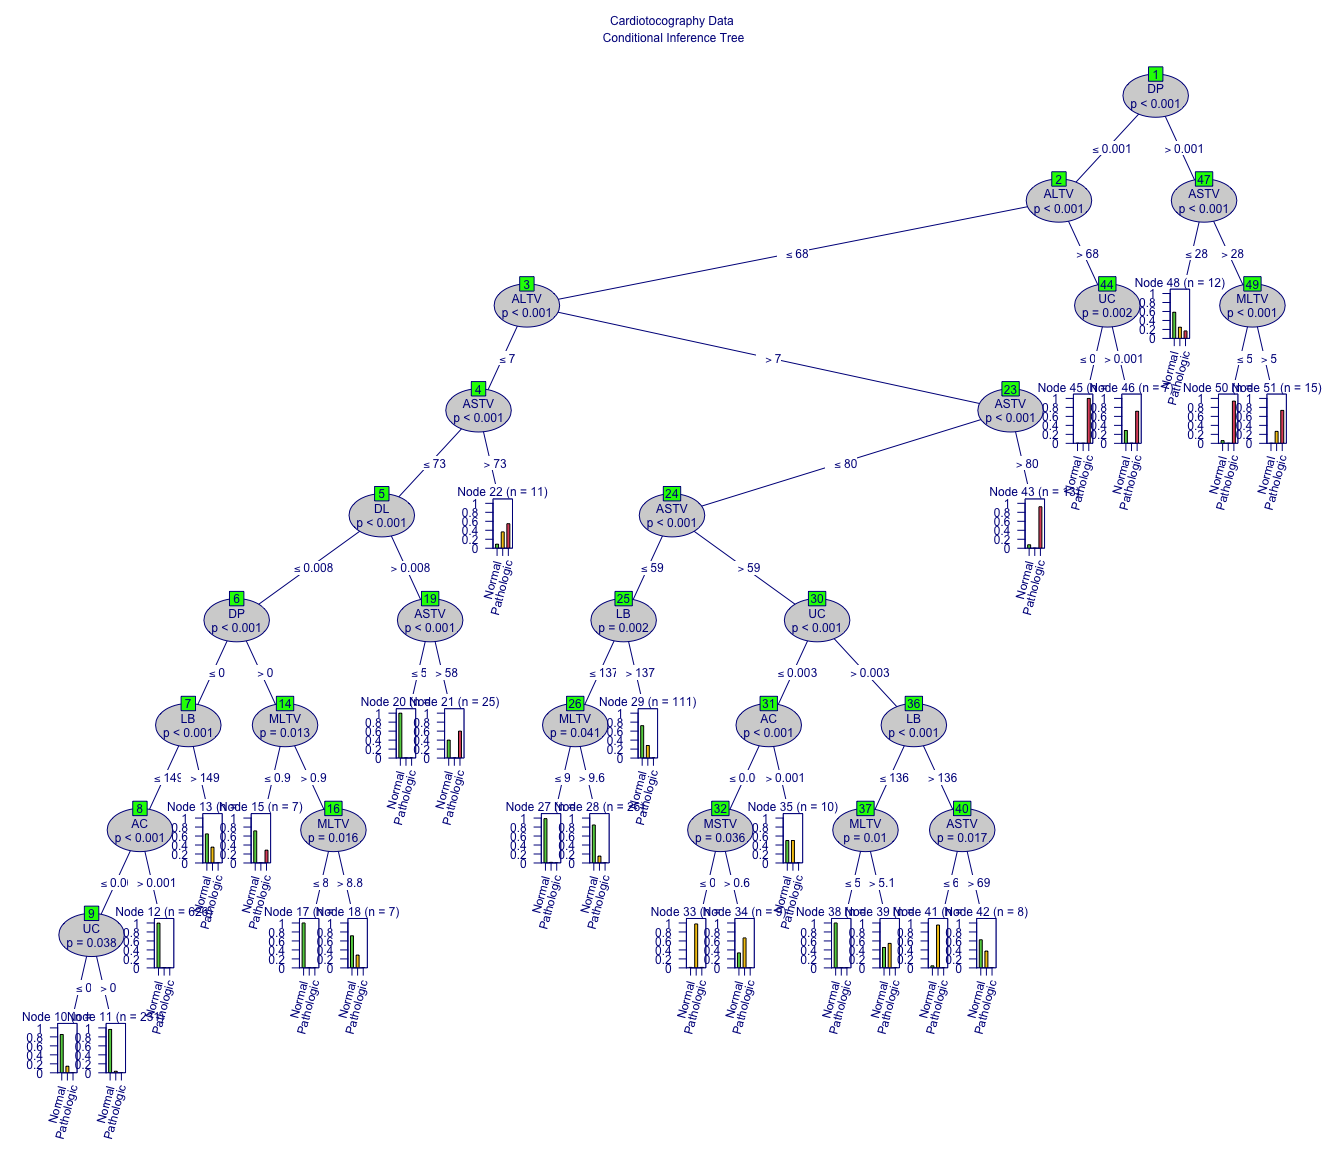
\includegraphics{CTREE_RMarkdown_files/figure-latex/viz-1.pdf}

\emph{Structure of training dataset model.}

The following confusion matrix illustrates how the model performed
against the training data. Out of 1523 total observations, the model
properly categorized 1413 for a predicted classification accuracy of
\textasciitilde93\%.

\begin{verbatim}
##             ACTUAL
## PREDICTED    Normal Suspect Pathologic
##   Normal       1168      70          4
##   Suspect        10     123          1
##   Pathologic     17       8        122
\end{verbatim}

\begin{verbatim}
## [1] 0.9277741
\end{verbatim}

\begin{verbatim}
##             ACTUAL
## PREDICTED          Normal      Suspect   Pathologic
##   Normal     0.7669074196 0.0459619173 0.0026263953
##   Suspect    0.0065659882 0.0807616546 0.0006565988
##   Pathologic 0.0111621799 0.0052527905 0.0801050558
\end{verbatim}

\emph{Figure 2.2 -- Training model confusion matrix.}

\textbf{Findings:}

Completed the training portion, the test sample was evaluated against
the model.As mentioned before, this set contained the remaining 30\% of
the sampled population. The same branched out to 16 inner nodes and 17
leaf nodes, for a total of 33. Nodes 33, 32, 30, 28, 18, 17, and 15 were
distinguished by containing observations identified as pathologic.
Alternatively, node 27, 24, and 14 predominant classification was
suspect. Refer to appendix A5 for a full depiction of this model in
``simple'' mode.

\emph{Figure 2.4 -- Structure of test data model.}

\begin{Shaded}
\begin{Highlighting}[]
\FunctionTok{plot}\NormalTok{(model2, }\AttributeTok{ep\_args =} \FunctionTok{list}\NormalTok{(}\AttributeTok{justmin =} \DecValTok{10}\NormalTok{), }\AttributeTok{type=}\StringTok{"extended"}\NormalTok{, }\AttributeTok{drop\_terminal =}\NormalTok{ T, }
     \AttributeTok{tnex=}\FloatTok{1.2}\NormalTok{, }\AttributeTok{gp=} \FunctionTok{gpar}\NormalTok{(}\AttributeTok{fontsize =} \DecValTok{10}\NormalTok{, }\AttributeTok{col=}\StringTok{"dark blue"}\NormalTok{), }
     \AttributeTok{inner\_panel =} \FunctionTok{node\_inner}\NormalTok{ (model2, }\AttributeTok{fill=}\FunctionTok{c}\NormalTok{(}\StringTok{"lightgrey"}\NormalTok{,}\StringTok{"yellow"}\NormalTok{), }\AttributeTok{pval=}\ConstantTok{TRUE}\NormalTok{, }\AttributeTok{id=}\ConstantTok{TRUE}\NormalTok{),}
     \AttributeTok{terminal\_panel=}\FunctionTok{node\_barplot}\NormalTok{(model2, }\AttributeTok{col=}\StringTok{"black"}\NormalTok{, }\AttributeTok{fill=}\FunctionTok{c}\NormalTok{(}\DecValTok{3}\NormalTok{,}\DecValTok{7}\NormalTok{,}\DecValTok{2}\NormalTok{, }\FloatTok{0.3}\NormalTok{), }\AttributeTok{beside=}\ConstantTok{TRUE}\NormalTok{, }
     \AttributeTok{ymax=}\DecValTok{1}\NormalTok{, }\AttributeTok{rot =} \DecValTok{90}\NormalTok{, }\AttributeTok{just =} \FunctionTok{c}\NormalTok{(}\StringTok{"right"}\NormalTok{, }\StringTok{"top"}\NormalTok{), }\AttributeTok{ylines=}\NormalTok{T, }
     \AttributeTok{widths=}\DecValTok{1}\NormalTok{, }\AttributeTok{gap=}\FloatTok{0.1}\NormalTok{, }\AttributeTok{reverse=}\ConstantTok{FALSE}\NormalTok{, }\AttributeTok{id=}\ConstantTok{TRUE}\NormalTok{), }\AttributeTok{margins =} \FunctionTok{c}\NormalTok{(}\DecValTok{5}\NormalTok{, }\DecValTok{3}\NormalTok{, }\DecValTok{4}\NormalTok{, }\DecValTok{2}\NormalTok{), }
     \AttributeTok{main=}\StringTok{"Cardiotocography Data}\SpecialCharTok{\textbackslash{}n}\StringTok{ Extended Conditional Inference Tree"}\NormalTok{)}
\end{Highlighting}
\end{Shaded}

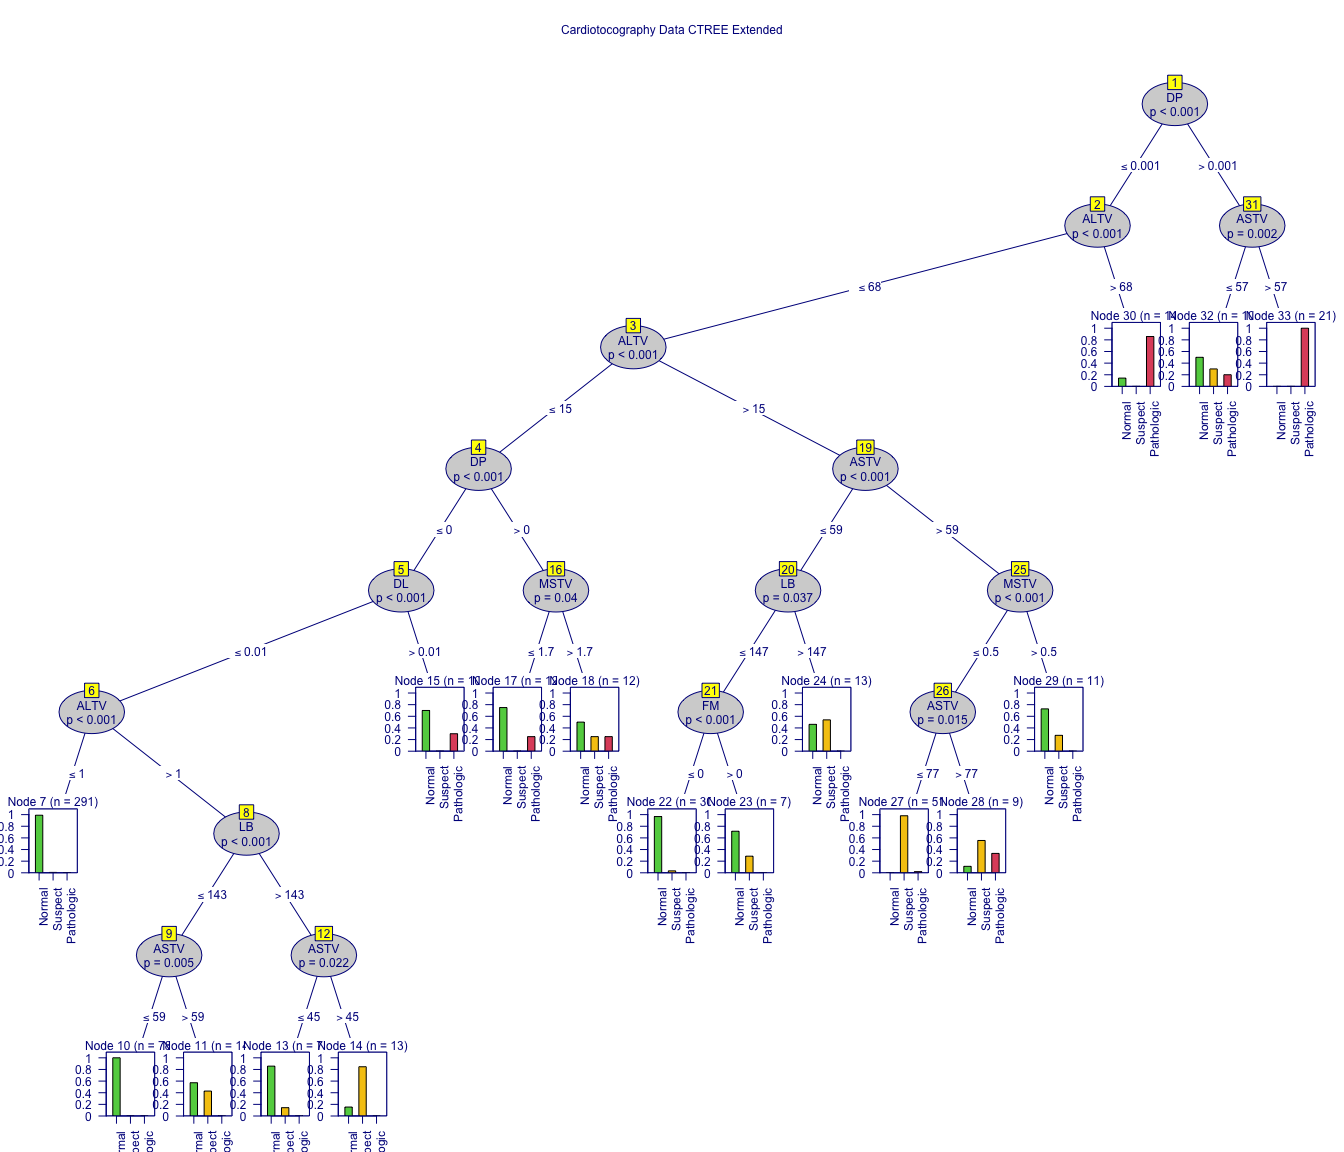
\includegraphics{CTREE_RMarkdown_files/figure-latex/unnamed-chunk-1-1.pdf}

\emph{Figure 2.5 -- Test data conditional inference tree.}

Per the above graphic (figure 2.5), variables prolonged decelerations
(DP), percentage of time with abnormal long term variability (ALTV), and
percentage of time with abnormal short term variability (ASTV) were key
splitting nodes affecting all other child-nodes. The data does not
provide the causes of these irregularities, but it does highly the
important of such percentages as triggers to constantly observe.
Importantly, node 5 portrays a split based on FHR baseline changes (DL).
It segregates readings based on those bellow or above the 1\% variation.
Those greater than or equal to 0.01 branch out to terminal node 15,
including pathologic readings. On the other side, those less than or
equal to 0.01 branch to the left. This node 5 splitting point, captures
403 out of the 637 sample for a total of 64.5\% (including node 15)
based on the DL reading, highlighting the previously mentioned
assumption on the importance of those DL readings within 2 standard
deviations. The confusion matrix for the test.data model captures a
total of 555 correct predictions for a classification accuracy rate of
92\% with confidence intervals between 89.5\% and 94\%.

\begin{Shaded}
\begin{Highlighting}[]
\CommentTok{\# Confusion matrix and stats}
\NormalTok{testPred2 }\OtherTok{\textless{}{-}} \FunctionTok{predict}\NormalTok{(model2, }\AttributeTok{newdata =}\NormalTok{ test.data, }\AttributeTok{method=}\StringTok{"NSP"}\NormalTok{)}
\FunctionTok{confusionMatrix}\NormalTok{(testPred2, test.data}\SpecialCharTok{$}\NormalTok{NSP)}
\end{Highlighting}
\end{Shaded}

\begin{verbatim}
## Confusion Matrix and Statistics
## 
##             Reference
## Prediction   Normal Suspect Pathologic
##   Normal        449      21         12
##   Suspect         9      73          4
##   Pathologic      2       0         33
## 
## Overall Statistics
##                                           
##                Accuracy : 0.9204          
##                  95% CI : (0.8958, 0.9407)
##     No Information Rate : 0.7629          
##     P-Value [Acc > NIR] : < 2.2e-16       
##                                           
##                   Kappa : 0.7809          
##                                           
##  Mcnemar's Test P-Value : 0.001165        
## 
## Statistics by Class:
## 
##                      Class: Normal Class: Suspect Class: Pathologic
## Sensitivity                 0.9761         0.7766           0.67347
## Specificity                 0.7692         0.9745           0.99639
## Pos Pred Value              0.9315         0.8488           0.94286
## Neg Pred Value              0.9091         0.9594           0.97183
## Prevalence                  0.7629         0.1559           0.08126
## Detection Rate              0.7446         0.1211           0.05473
## Detection Prevalence        0.7993         0.1426           0.05804
## Balanced Accuracy           0.8727         0.8755           0.83493
\end{verbatim}

\emph{Figure 2.6 -- Test data sample confusion matrix.}

\begin{center}\rule{0.5\linewidth}{0.5pt}\end{center}

\textbf{Conclusion:}

Based on the above model's descriptions, and inferred findings, one may
argue and advocate for the use of supervised learning algorithms, like
the ctree. This can definitely serve as supporting mechanisms through
the medical industry, especially, as evaluated here neonatal, or labor
and delivery medical departments. Per the described intended goals, this
study employed the ctree methodology to assess and classified
independent variables and their influence toward the response variable
of NSP. As previously alluded, the model enhances uncovering
inclinations, branches, or tree nodes not typically perceivable by the
human naked-eye, thus discourages the practice of CTG interpretation
solely based on the medical practitioner experience. Although this is a
basic assessment on the usability of the ctree algorithm, supplemented
with other data mining techniques including, but not limited to,
clustering, classification and dimensionality reduction, could boost the
performance accuracy of the model while reducing error variances. Some
encountered challenges while conducting the study were related to
identifying best transformation techniques or interpretation of the
data, given the limited background of the medial domain. As a
recommendation, any future development of this algorithm in relation to
CTGs would highly benefit from having sustainable knowledge of this
medial area. For best accuracy outcomes, better transformation
techniques and variable selection process is essential.

\begin{center}\rule{0.5\linewidth}{0.5pt}\end{center}

\textbf{Note:} The \texttt{echo\ =\ FALSE} parameter was added to the
code chunks to prevent printing of the underpining R code.

\end{document}
